\section{Proposta}

\begin{frame}{range min-Max tree k-ária (rmM-tree k-ária)}
    Características:
        \begin{itemize}
            \item Alto fator de ramificação;
            \item Maior cobertura de área por nó;
            \item Cada nó cobre até $k$ intervalos;
            \item Mesmas definições de registros da estrutura binária;
            \item Complexidade de tempo e espaço eficientes, usando os mesmos campos defindos por \cite{book-compact-data-structures} em sua estrutura.
        \end{itemize}
\end{frame}

\begin{frame}{rmM-tree k-ária}
    \textbf{Árvore de entrada}
        \begin{figure}[h!]
            \centering
            
            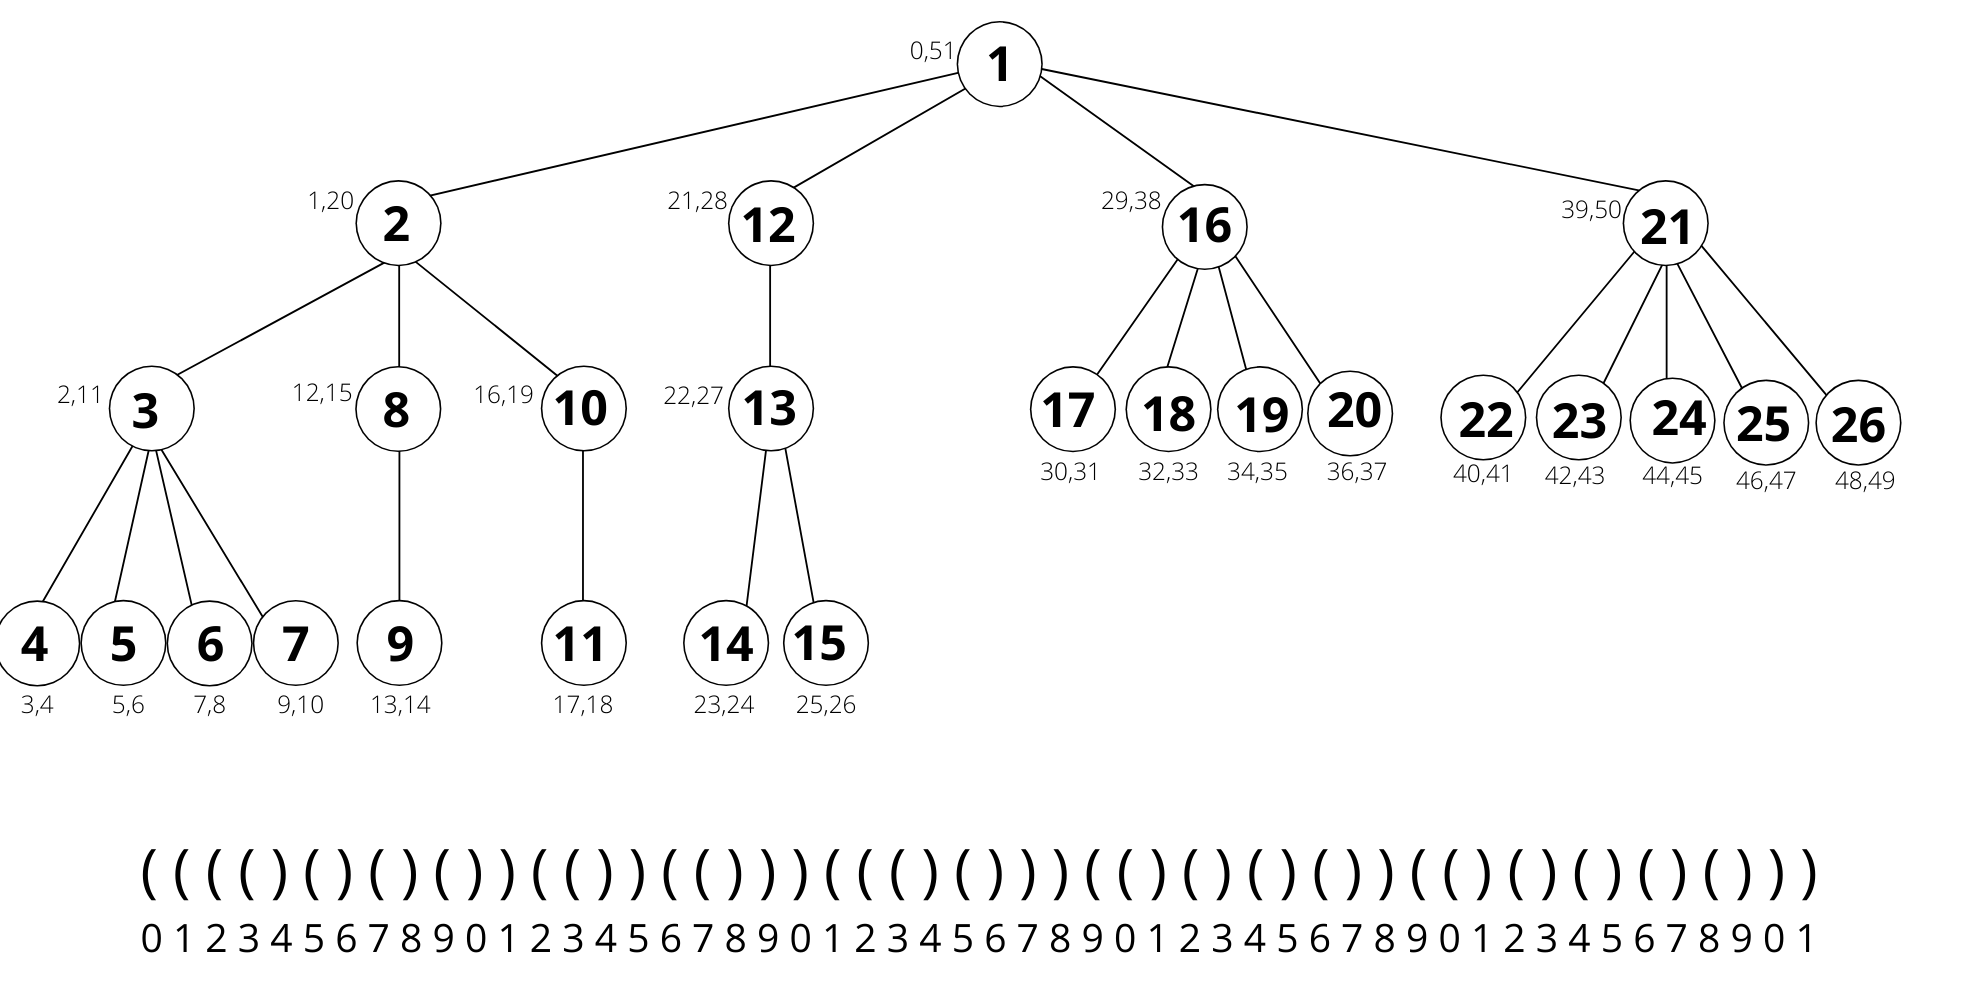
\includegraphics[scale=0.37]{images/arvore_geral.png}
        \end{figure} 
\end{frame}

\begin{frame}{rmM-tree k-ária: Registros}
    \begin{figure}[h!]
        \centering
        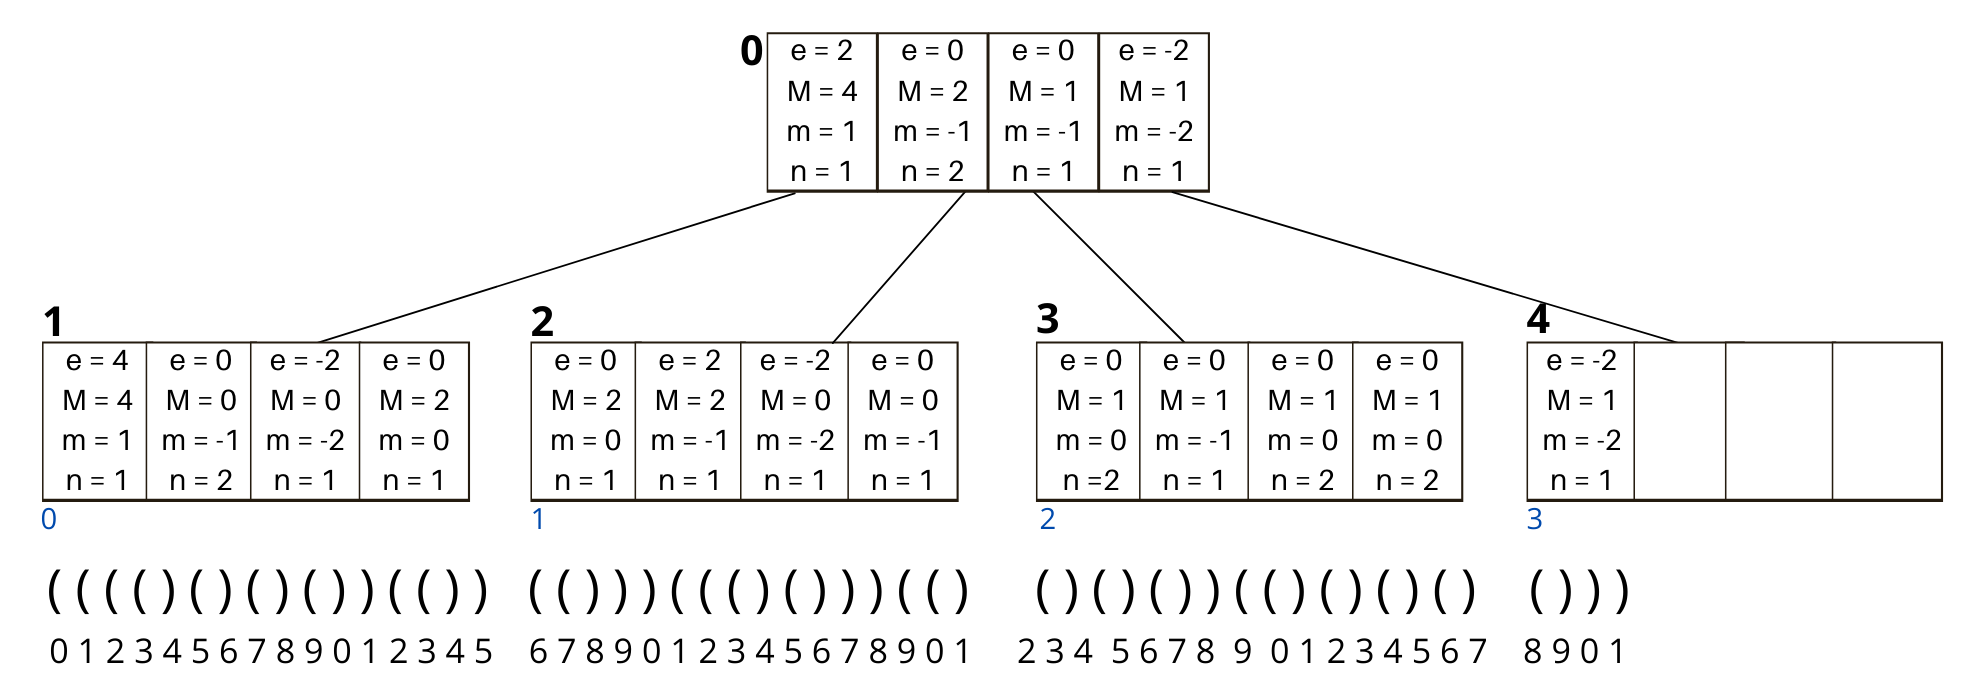
\includegraphics[scale=0.4]{images/rmm-tree-kary.png}\\
        \caption{rmM-tree 4-ária com blocos de tamanho 4}
    \end{figure} 
\end{frame}

\begin{frame}{rmM-tree k-ária: Registros}
    \textbf{Nós internos e raíz}
    \begin{figure}[h]
        \begin{minipage}[c]{0.25\linewidth}
            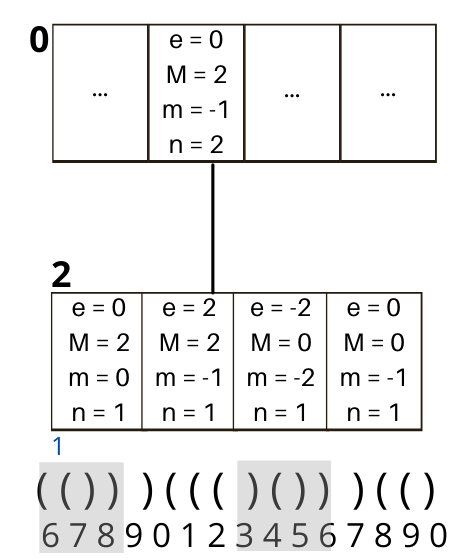
\includegraphics[scale=0.70]{images/k-internal-nodes.png}
        \end{minipage}
        \begin{minipage}[c]{0.70\linewidth}
                \begin{eqnarray*}
                    \begin{split}
                        R[0][1].M =& max(R[2][0].M, \\
                        &   R[2][0].e + R[2][1].M, \\
                        &   R[2][0].e + R[2][1].e + R[2][2].M,  \\
                        &   R[2][0].e + R[2][1].e + R[2][2].e  +\\
                        &   R[2][3].M)\\
                        &   = max(2,2,2,0) = 2;
                    \end{split}
                \end{eqnarray*}
        \end{minipage}
    \end{figure}
\end{frame}

\begin{frame}{rmM-tree k-ary: Operações}
    \begin{table}
        \centering
        \caption[Operações sobre a rmM-tree binária e k-ária]{Operações suportadas pela rmM-tree binária e rmM-tree-kária}
	    \resizebox{\columnwidth}{!}{
            \begin{tabular}{|c|c|c|}
                \hline
                \textbf{Operação} & \textbf{rmM-tree binária} & \textbf{rmM-tree k-ária}\\ \hline
                fwdSearch(i,d)  &  \cmark \par &   \cmark \par\\ \hline
                bwdSearch(i,d)  &  \cmark \par &   \cmark \par\\ \hline
                minExcess(i,j) / maxExcess(i,j)  &   \cmark \par & \xmark \\ \hline
                minCount(i,j)  &   \cmark \par & \xmark\\ \hline
                minSelectExcess(i,j,t)  &  \cmark \par & \xmark\\ \hline
                enclose(i) &  \cmark \par &   \cmark \par \\ \hline
                rmq(i,j) / rMq(i,j) &  \cmark \par & \xmark \\ \hline
                rank$_1$(i) / rank$_0$(i) &  \cmark \par &    \cmark \par\\ \hline
                select$_1$(i) / select$_0$(i) &  \cmark \par &   \cmark \par\\ \hline
            \end{tabular}
        }
    \end{table}
\end{frame}

\begin{frame}{rmM-tree k-ary: Operações}
    \begin{table}
        \centering
        \caption[Operações sobre a rmM-tree binária e k-ária]{Operações suportadas pela rmM-tree binária e rmM-tree-kária}
	    \resizebox{\columnwidth}{!}{
            \begin{tabular}{|c|c|c|}
                \hline
                \textbf{Operação} & \textbf{rmM-tree binária} & \textbf{rmM-tree k-ária}\\ \hline
                preRank(i)/postRank(i) &  \cmark \par &   \cmark \par\\ \hline
                preSelect(i)/postSelect(i) &  \cmark \par &   \cmark \par \\ \hline
                isLeaf(i) &  \cmark \par &   \cmark \par\\ \hline
                isAncestor(i,j) &  \cmark \par &   \cmark \par\\ \hline
                depth(i) &   \cmark \par &   \cmark \par\\ \hline
                parent(i) &  \cmark \par &   \cmark \par\\ \hline
                firstChild(i) / lastChild(i) &  \cmark \par &   \cmark \par\\ \hline
                child(i,t)&  \cmark \par & \xmark \\ \hline
                nextSibling(i) / prevSibling(i) &   \cmark \par &   \cmark \par\\ \hline
            \end{tabular}
        }
    \end{table}
\end{frame}

\begin{frame}{rmM-tree k-ary: Operações}
    \begin{table}
        \centering
        \caption[Operações sobre a rmM-tree binária e k-ária]{Operações suportadas pela rmM-tree binária e rmM-tree-kária}
	    \resizebox{\columnwidth}{!}{
            \begin{tabular}{|c|c|c|}
                \hline
                \textbf{Operação} & \textbf{rmM-tree binária} & \textbf{rmM-tree k-ária}\\ \hline
                subtreeSize(i) &   \cmark \par &   \cmark \par\\ \hline
                levelAncestor(i,d) &   \cmark \par &   \cmark \par \\ \hline
                levelNext(i) / levelPrev(i) &   \cmark \par &   \cmark \par \\ \hline
                levelLeftMost(d) / levelRightMost(d) &  \cmark \par &   \cmark \par\\ \hline
                lca(i,j)&  \cmark \par & \xmark\\ \hline
                deepestNode(i)&  \cmark \par & \xmark \\ \hline
                degree(i)&  \cmark \par & \xmark\\ \hline
                childRank(i)&  \cmark \par & \xmark\\ \hline
                leafRank(i)/leafSelect(i)&  \cmark \par  &   \cmark \par\\ \hline
                leftMostLeaf(i)/rightMostLeaf(i)&   \cmark \par &   \cmark \par\\ \hline
            \end{tabular}
        }
    \end{table}
\end{frame}


\begin{frame}{rmM-tree k-ary: operações}
    Problema: Dado um nó codificado em $i=1$, encontrar o nó codificado em $j>i$, mais à esquerda de $i$.

    Solução: 
    $$nextSibling(i) = findClose(i) +1$$ 
    $$findClose(i) = fwdSearch(i,-1)$$ 
 \end{frame}

 \begin{frame}{rmM-tree k-ary: $nextSibling$}
    Problema: Computar $nextSibling(1)$.
     \begin{figure}[h!]
         \centering
         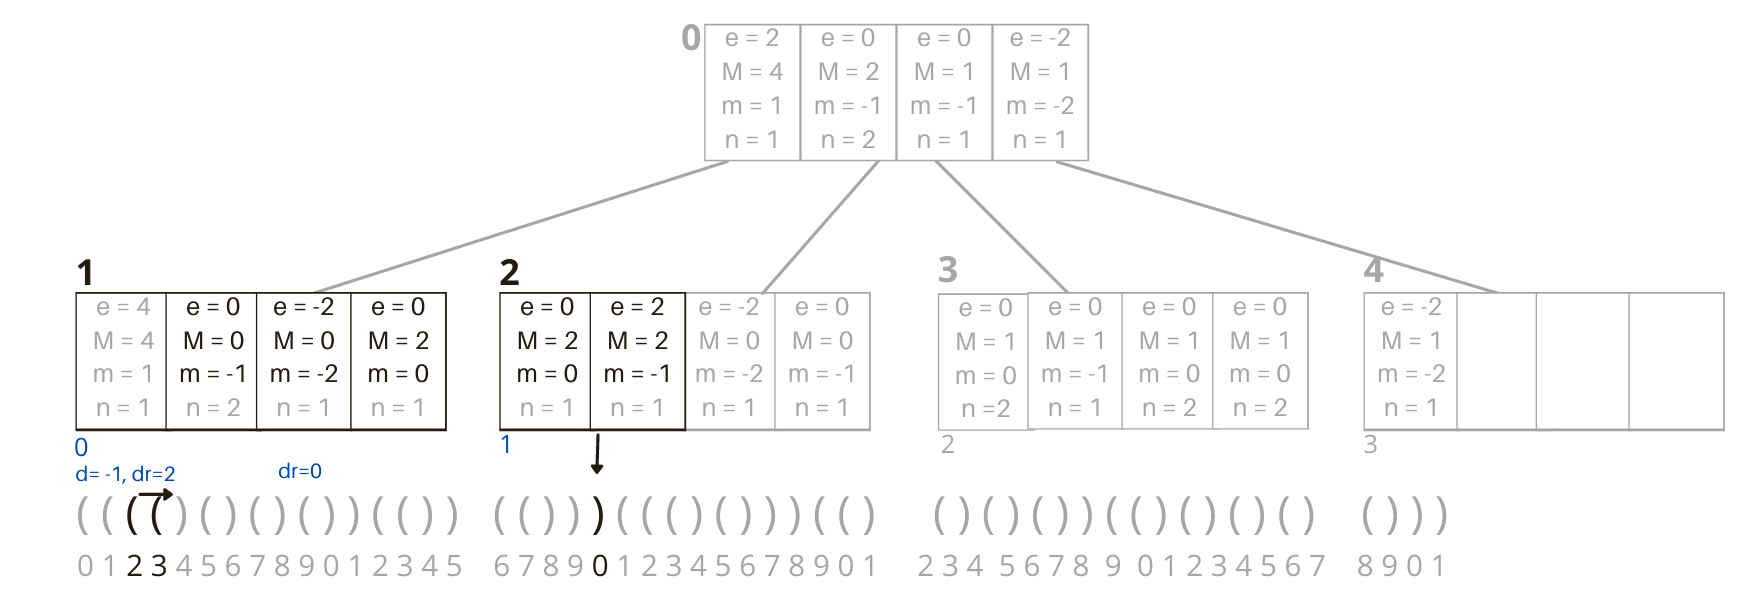
\includegraphics[scale=0.8]{images/rmm-tree-kary-fwd.png}\\
         \caption{Simulação de $fwdSearch(1,-1)=20$ em uma rmM-tree 4-ária}
     \end{figure} 
 \end{frame}

 \begin{frame}{rmM-tree k-ary: $nextSibling$}
    Problema: Computar $nextSibling(1)$.
     \begin{figure}[h!]
         \centering
         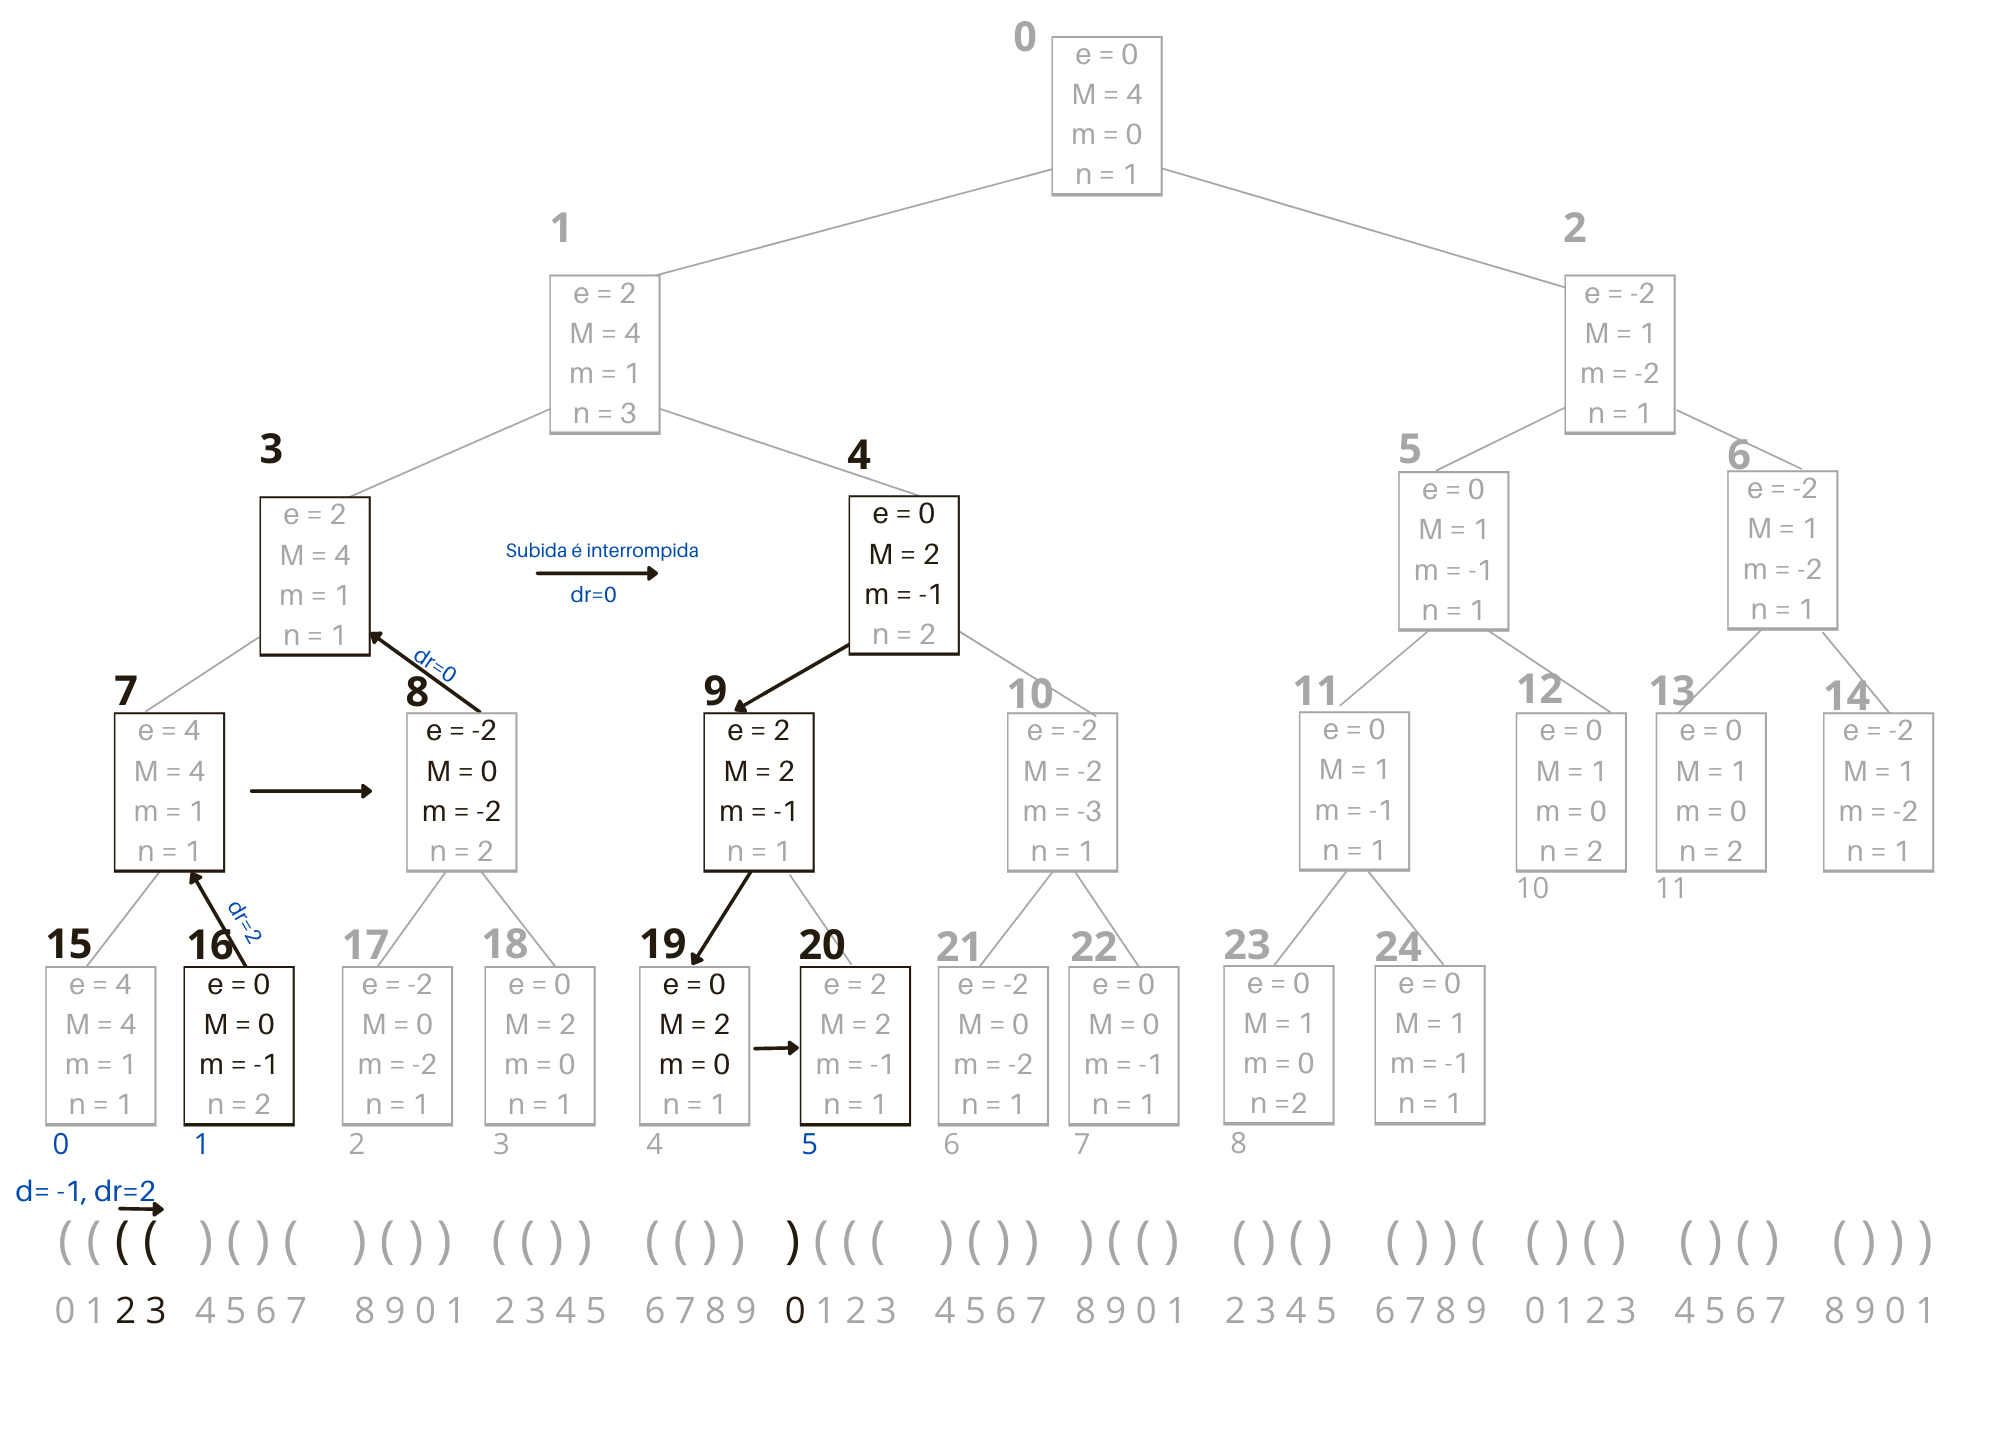
\includegraphics[scale=0.27]{images/rmm-tree-bin-fwdSearch.png}\\
         \caption{Simulação de $fwdSearch(1,-1)=20$ usando a rmM-tree binária}
     \end{figure} 
 \end{frame}


 \begin{frame}{rmM-tree k-ary: $nextSibling$}
    Problema: Dado um nó codificado em $i=1$, encontrar o nó codificado em $j>i$, mais à esquerda de $i$.

    Solução: 
    $$findClose(1) = fwdSearch(1,-1) = 20 $$ 
    $$nextSibling(1) = fwdSearch(1,-1) + 1 = 21 $$ 
 \end{frame}

 \begin{frame}{rmM-tree k-ary: $nextSibling$}
    Solução:  $nextSibling(1)$.
     \begin{figure}[h!]
         \centering
         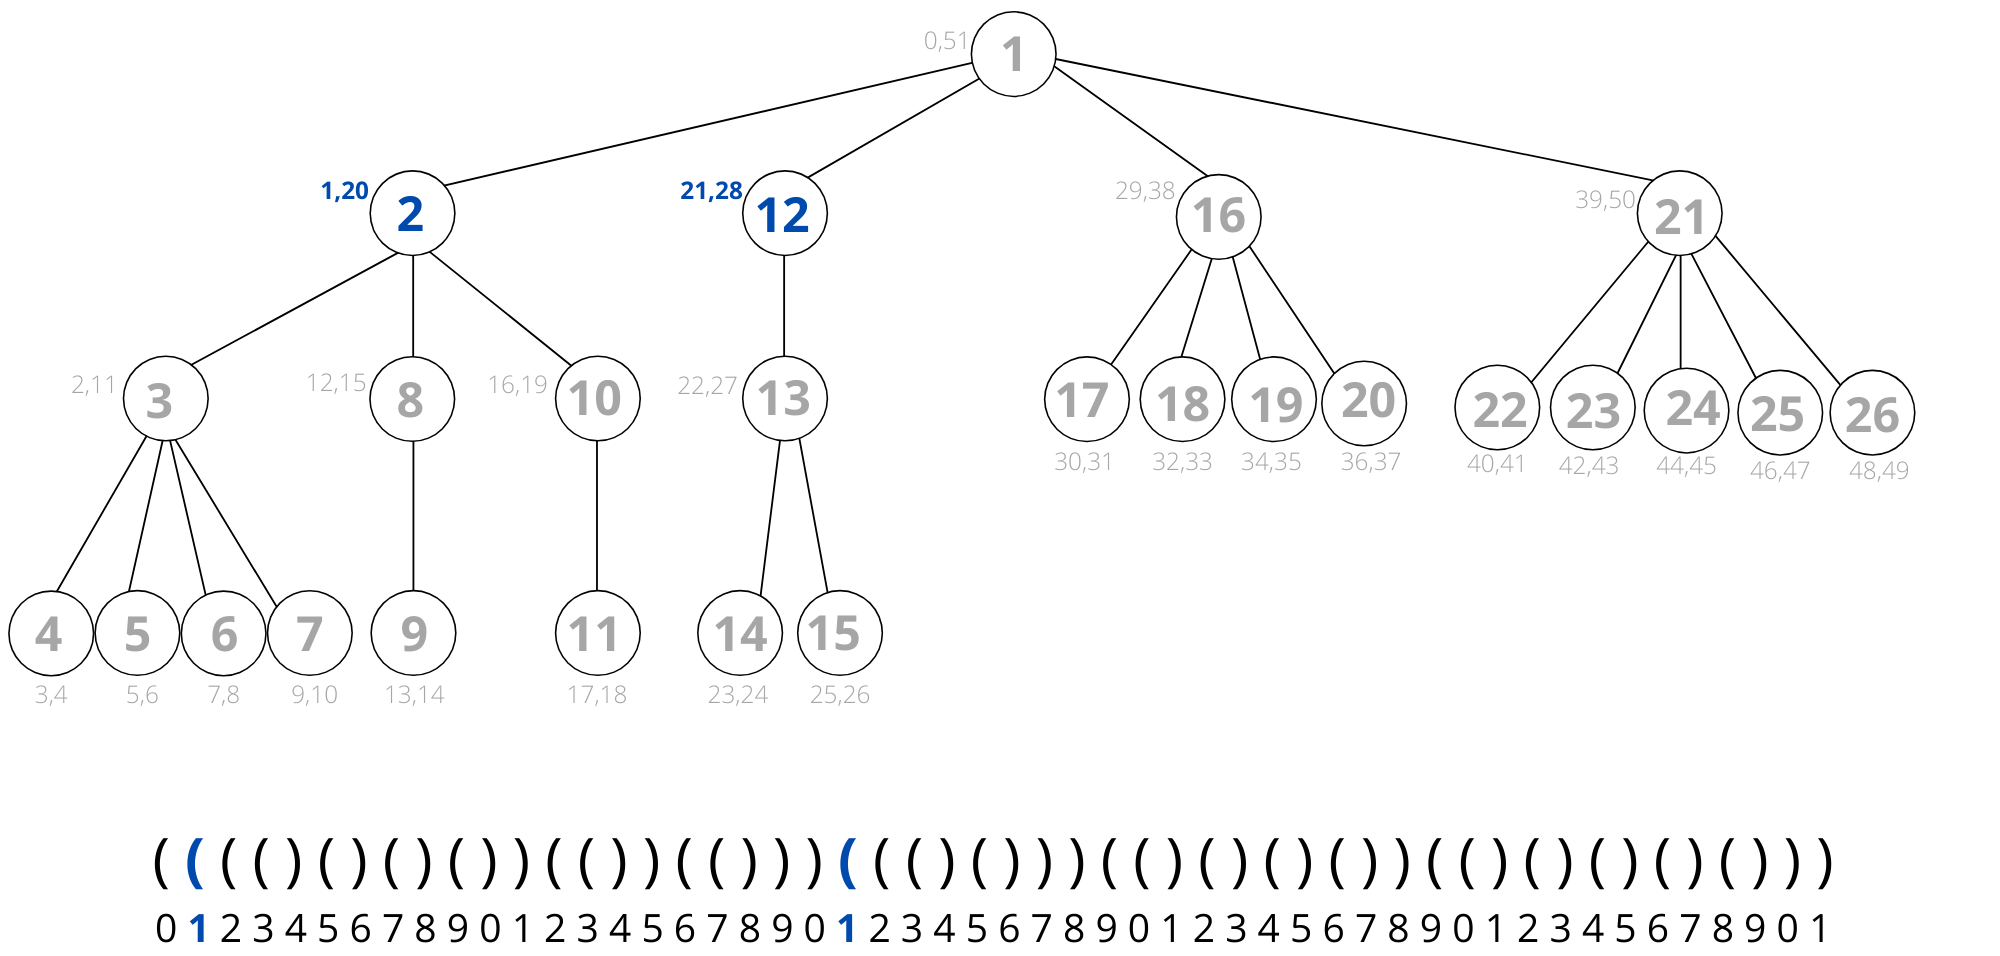
\includegraphics[scale=0.40]{images/nextSibling-res.png}\\
         \caption{Árvore de entrada}
     \end{figure} 
 \end{frame}